\documentclass{article}
\usepackage{fontspec}
\usepackage{polyglossia}
\setdefaultlanguage{french}
\usepackage[a4paper,margin=2.5cm]{geometry}

\usepackage{amsmath}
\usepackage{amssymb}
\usepackage{array}
\usepackage{auto-pst-pdf}
\usepackage{booktabs}
\usepackage{cite}
\usepackage{graphicx}
\usepackage{lmodern}
\usepackage{marvosym}
\usepackage{mathrsfs}
\usepackage{minted}
\usepackage{multicol}
\usepackage{multirow}
\usepackage{paralist}
\usepackage{schemabloc}
\usepackage{siunitx}
\usepackage{soul}
\usepackage{tikz}
\usepackage[european,americanresistors,cuteinductors,siunitx,arrowmos]{circuitikz}
\usepackage{url,hyperref}
\usepackage{verbatim}
\usepackage{xunicode,xltxtra}

\title{
\includegraphics{../../../images/inp-enseeiht} \\ ~ \\ ~ \\ ~ \\ ~ \\ Régulateur linéaire faible puissance et large bande}
\author{François Pierron \& Guilhem Saurel}
\date{\oldstylenums{\today}}

\begin{document}

\begin{titlepage}
    \setcounter{page}{0}
    \maketitle
    \vfill
    \tableofcontents
    \thispagestyle{empty}
\end{titlepage}

\section*{Introduction}

l’objectif de ce BE est de concevoir et de simuler un ASIC analogique, d’abord en schématique avec Orcad et Spice puis en layout avec Cadence.

~

Le sujet proposé est la conception d’une alimentation stabilisée, composée d’un band-gap et d’un amplificateur différentiel. Nous traiterons la seconde partie, mais en prenant soin de nous intéresser à ce qu’au moins l’un des autres binôme aura comme résultats pour le band-gap, notamment en ce qui concerne leur tension de sortie, puisque c’est notre tension d’entrée, ainsi qu’au niveau de leur consommation, vu que c’est la consommation globale du système qui est à prendre en compte

~

Aussi, si nous avons le temps, ça serait intéressant de faire un routage et une simulation en layout complète avec les deux sous-systèmes.

\section{Architecture}

\subsection{Vue d’ensemble}

\begin{center}\begin{circuitikz} \draw
    (0,0) node[draw, minimum size=2em] (bg) {Band-gap}
    (0,1) node[sground, rotate=180] {} -- (bg.north)
    (0,-1) node[ground] {} -- (bg.south)
    (4,-0.5) node[op amp, yscale=-1] (oa) {}
    (oa.+) to[short, l_=$V_{ref}$] (bg.east)
    (7,-0.5) node[nmos] (ballast) {ballast}
    (ballast.gate) to[short, l_=$V_g$] (oa.out)
    (7,1) node[sground, rotate=180] {} -- (ballast.drain)
    (ballast.source) -- (7,-2) to[short, l^=$V_{out}$] (9,-2) -- (10,-2) to[R=$R_{ch}$] (10,-6)
    (7,-2) to[R=$R_2$] (7,-4) to[R=$R_1$] (7,-6) node[ground] {} -- (10,-6)
    (9,-2) to[C,l_=$C_{ch}$] (9,-6)
    (7,-4) -- (2,-4) -- (2,-1) -- (oa.-)
; \end{circuitikz}\end{center}

Notre but est donc de partir d’un $V_{ref}$ censé être relativement stable à 1.24V pour obtenir une tension de sortie de 2V indépendante de la température et des problèmes qui peuvent survenir lors de la fabrication d’un ASIC.

Pour cela, on utilise un pont diviseur de tension censé passer le 2V à 1.24V, et on reboucle ce 1.24V vers l’entrée inverseuse de l’amplificateur opérationnel afin qu’à son tour il nous fournisse la tension de sortie de 2V.

~

Cependant, cet amplificateur opérationnel ne peut pas délivrer un courant de sortie suffisant, donc on ajoute un ballast dans la boucle.

~

Pour les simulations, le circuit sera chargé par un un circuit RC parallèle.

\subsection{Amplificateur Opérationnel}

Pour la conception de cet amplificateur opérationnel, nous utiliserons simplement une paire différentielle suivie d’un étage d’amplifaction en source commune.

\newpage

\section{Conception et simulations sous Orcad \& PSpice}

Dans un premier temps, nous allons simuler un circuit sans tenir compte des contraintes de fabrication, où les transistors doivent être appairés, où les résistances doivent avoir des valeurs proches, etc.

\subsection{Schématique de l’ASIC}

On se rend compte que notre gain n’est pas tout à fait satisfaisant, donc pour l’augmenter nous cascodons l’étage d’amplification.

Les cascodes ayant besoin d’une tension de polarisation, nous ajoutons également deux branches composées de transdiodes calibrées de manière à obtenir les tensions de polarisation nécessaires.

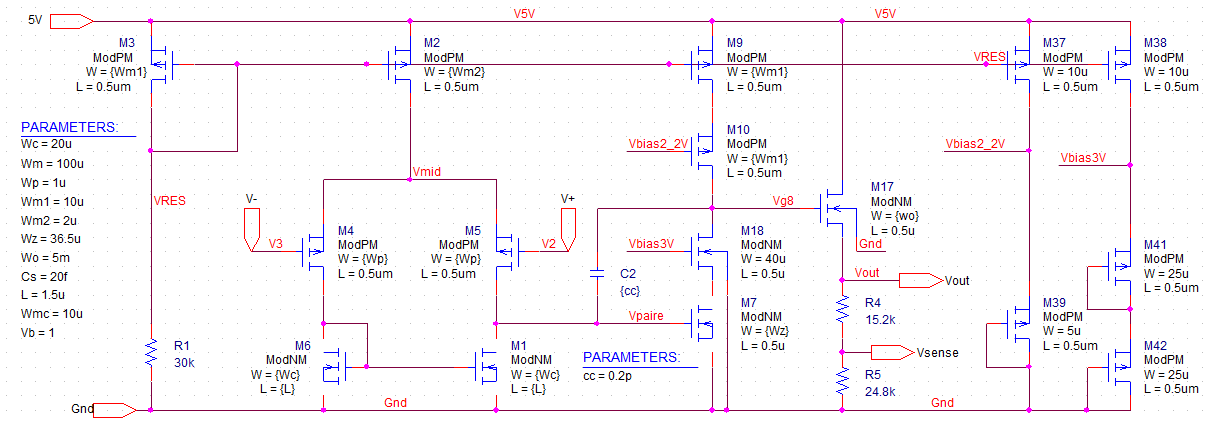
\includegraphics[width=\linewidth]{schema_asic.png}

\subsection{Circuits de simulation}

Pour mesurer les différentes performances de notre circuit, nous avons du créer plusieurs schéma de niveau hiérarchique supérieur.

Ils sont relativement similaires à celui-ci:

\begin{center}
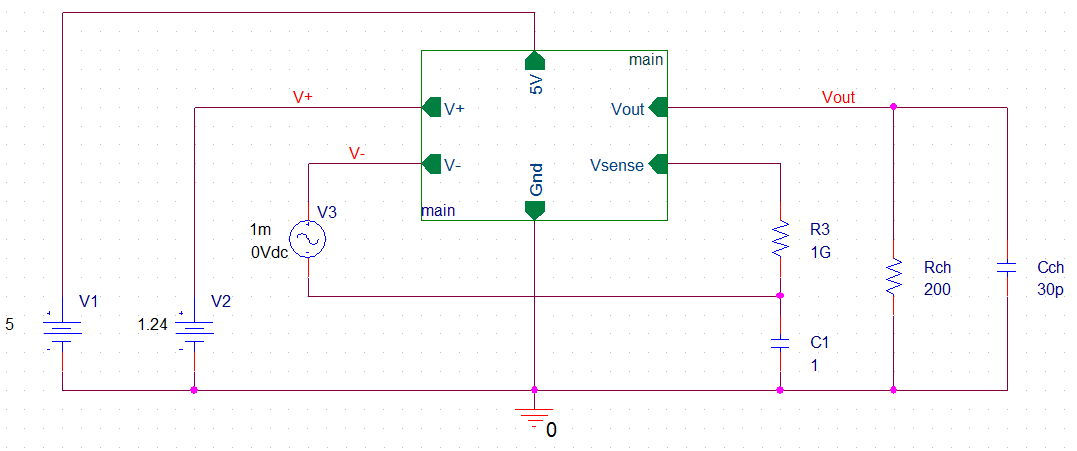
\includegraphics[width=\linewidth-5cm]{schema_bode.png}
\end{center}

Voici un diagramme de Bode typiquement obtenu lors des simulations:

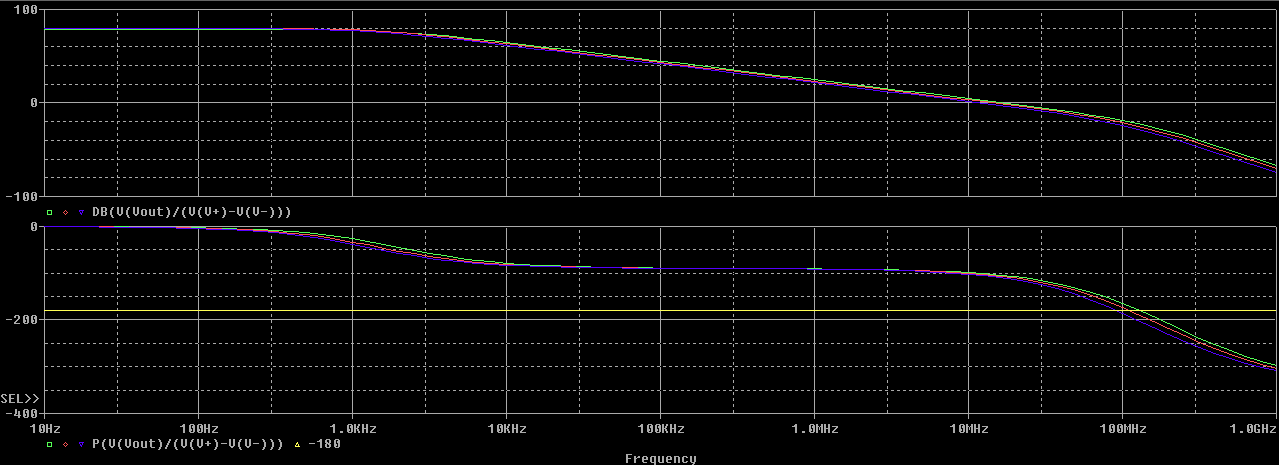
\includegraphics[width=\linewidth]{bode_typique.png}

\subsection{Résultats}

En analysant le diagramme de Bode et d’autres simulations, nous pouvons obtenir les différents résultats nous intéressant, pour plusieurs températures.

\subsubsection{Typique}

\begin{center}
\begin{tabular}{|l|c|r|r|r|}
    \hline
    Paramètre & Unité & T=-40°C & T=27°C & T=125°C \\
    \hline
    Marge de phase & degrès & 75.1 & 75.3 & 75.3 \\
    \hline
    Marge de gain & dB & 22.6 & 22.6 & 22.7 \\
    \hline
    Gain & dB & 78.6 & 79.7 & 79.1 \\
    \hline
    Offset & µV & -28.7 & 11.3 & 32.3 \\
    \hline
    PSSR & dB & 97.7 & 84.4 & 79 \\
    \hline
    Consommation & µA & 497 & 500.5 & 508 \\
    \hline
    Impédance de sortie & Ω & 5.92 & 6.99 & 8.47 \\
    \hline
\end{tabular}
\end{center}

Ces résultats typiques ne nous suffisent pas, puisqu’il faut prendre en compte toutes les parties aléatoires du process technologique. Nous répétons donc toutes ces simulations avec différents modèles de transistors dégradés fournis par le fondeur afin d’avoir la certitude que notre circuit remplira ses objectif quelques soient les problèmes rencontrés lors de la fabrication.

\subsubsection{Dégradés}

\begin{center}
\begin{tabular}{|l|c|r|r|r|}
    \hline
    \multicolumn{5}{|c|}{\textbf{Worst One}}\\
    \hline
    Paramètre & Unité & T=-40°C & T=27°C & T=125°C \\
    \hline
    Marge de phase & degrès & 79.4 & 79.6 & 79.3 \\
    \hline
    Marge de gain & dB & 24.7 & 24.7 & 24.5 \\
    \hline
    Gain & dB & 86.2 & 82.9 & 74.4 \\
    \hline
    Offset & µV & 9.84 & 10.6 & 12.4 \\
    \hline
    PSSR & dB & 53 & 53.5 & 56.3 \\
    \hline
    Consommation & µA & 458 & 460 & 462 \\
    \hline
    Impédance de sortie & Ω & 5.38 & 6.33 & 7.75 \\
    \hline
    \multicolumn{5}{|c|}{\textbf{Worst Power}}\\
    \hline
    Paramètre & Unité & T=-40°C & T=27°C & T=125°C \\
    \hline
    Marge de phase & degrès & 75.8 & 76.1 & 76.1 \\
    \hline
    Marge de gain & dB & 21.3 & 21.4 & 21.3 \\
    \hline
    Gain & dB & 83.1 & 82.6 & 80.5 \\
    \hline
    Offset & µV & 10.9 & 11.7 & 12.9 \\
    \hline
    PSSR & dB & 52.7 & 52 & 51.2 \\
    \hline
    Consommation & µA & 559 & 562 & 569 \\
    \hline
    Impédance de sortie & Ω & 5.24 & 6.13 & 7.52 \\
    \hline
    \multicolumn{5}{|c|}{\textbf{Worst Speed}}\\
    \hline
    Paramètre & Unité & T=-40°C & T=27°C & T=125°C \\
    \hline
    Marge de phase & degrès & 75 & 75 & 74.5 \\
    \hline
    Marge de gain & dB & 24 & 24 & 23.8 \\
    \hline
    Gain & dB & 70.2 & 65.9 & 64 \\
    \hline
    Offset & µV & 4.34 & 4.41 & 4.34 \\
    \hline
    PSSR & dB & 55.7 & 51.8 & 50.004 \\
    \hline
    Consommation & µA & 450 & 449 & 449 \\
    \hline
    Impédance de sortie & Ω & 6.90 & 8.26 & 7.41 \\
    \hline
    \multicolumn{5}{|c|}{\textbf{Worst Zero}}\\
    \hline
    Paramètre & Unité & T=-40°C & T=27°C & T=125°C \\
    \hline
    Marge de phase & degrès & 69.6 & 69.9 & 70.1 \\
    \hline
    Marge de gain & dB & 20.6 & 20.7 & 20.7 \\
    \hline
    Gain & dB & 61.3 & 61.7 & 62 \\
    \hline
    Offset & µV & 5.6 & 5.9 & 6.2 \\
    \hline
    PSSR & dB & 55.5 & 55.8 & 56 \\
    \hline
    Consommation & µA & 547 & 551 & 558 \\
    \hline
    Impédance de sortie & Ω & 6.71 & 8.00 & 9.71 \\
    \hline
\end{tabular}
\end{center}

\subsubsection{Pire cas}

Une fois qu’on a déterminé les quatre pires cas en fabrication, on peut rechercher dans ces résultats les plus défavorables:

\begin{center}
\begin{tabular}{|l|c|r|}
    \hline
    Paramètre & Unité & \\
    \hline
    Marge de phase & degrès & 69.6 \\
    \hline
    Marge de gain & dB & 20.6 \\
    \hline
    Gain & dB &  61.3 \\
    \hline
    Offset & µV & 32.3 \\
    \hline
    PSSR & dB & 50.004 \\
    \hline
    Consommation & µA & 569 \\
    \hline
    Impédance de sortie & Ω & 9.71 \\
    \hline
\end{tabular}
\end{center}

On vient donc de vérifier que l’on entre dans tous les cas dans le cahier des charges (quoi que l’on soit un peu juste sur le PSSR dans le pire cas).

On peut donc passer sous Cadence pour router notre ASIC et le simuler à nouveau.

\section{Cadence}

\subsection{Conception du layout}

Chaque transistor a ici été découpé en plusieurs sous-parties, afin d’avoir des transistors tous de la même taille lorsqu’ils sont censés être appairés.

~

Il faut ensuite les répartir de manière à ce qu’un gradient de température ou de dopage les affecte tous de la même manière.

~

Il est donc indispensable de réfléchir à la forme données aux mirroirs de courant, puisque nous avons 1 + 5 + 5 transistors appairés.

Pour cela, on place logiquement celui qui est tout seul au centre de la structure, tandis que les 10 autres sont répartis autour et de manière alternée.

~

Pour les autres transistors appairés deux à deux, nous utileserons une structure classique en croix, où chaque transistor est scindé en deux.

~

On doit aussi prendre en compte la taille des grilles, car si elles sont trop longues, une différence de tension pourrait apparaître entre un bout et l’autre. On n’hésite donc pas à mettre plusieurs grilles, voire même découper le transistor en quatre parties lorsqu’il s’agit du ballast, qui est particulièrement volumineux.

~

Il est également indispensable d’ajouter un «Guard Ring» sur tous les MOSP puisqu’ils ont besoin d’un N-tub, vu que le substrat est de type P.

~

On se concentre aussi sur l’espace occupé total, qui doit être le plus petit possible afin d’avoir un composant final moins cher.

\newpage

\subsection{Conception du pont diviseur}

Après avoir discuté avec un autre binôme ayant eu la charge du band-gap, nous avons appris que leur tension de sortie était de 1.207V.

On doit donc faire un pont diviseur pour passer d’une tension la plus proche possible de 2V à une tension la plus proche possible de 1.207V.

~

Il y a également une contrainte importante au niveau des résistances qui doivent être toutes à peu près égales, sinon elles ne seraient pas affectées de la même manière lors d’un léger soucis de fabrication (ce qui arrivera forcément).

En effet, on a surtout besoin que le ratio entre ces différentes résistances reste le même, même si leurs valeurs changent.

~

Par exemple, si une résistance fait 2µm et une autre 1µm, et que le masque se désaligne de 0.1µm dans la direction des résistances, la valeur de la première serait affectée de 5\% et celle de la seconde de 10\%.

~

Pour parvenir à cet objectif, il nous faut d’abord imaginer une topologie cohérente avec N résistances en haut du pont diviseur et M résistance en bas. On remarque alors que $1.207\simeq1.2=\cfrac{3}{5}\times2$, donc on va partir sur N=3 et M=2.

La suite de l’exercice est laissée à un algorithme qui essaye un très grand nombre de valeurs possible pour les résistances du haut et celles du bas, en ne gardant que les couples de valeurs qui sont le plus proche possible de, et dont l’erreur obtenue est la plus faible possible. Une dernière contrainte porte sur le courant consommé, qui doit être de l’ordre de 50µA.

~

Notre choix s’arrête alors sur trois résistances en parallèle en haut du pont diviseur de 47580Ω et deux résistance en parallèle en bas de 48280Ω. Ces résistances ne sont différentes que de 1.44\%, et un tel pont diviseur nous fait passer de 2V à 1.207V avec une erreur de l’ordre de $3\cdot 10^{-6}$.

~

Il ne nous reste plus qu’à positioner ces cinq résistances de manière à ce qu’elles soient interlacées.

On rajoute également une résistance identique de chaque côté connectée à la masse, afin que les cinq résistances utiles voient la même chose à leur côté.

\newpage

\subsubsection{Layout}

Afin de rendre ce layout visible sur le papier, nous avons coupé le circuit en deux parties, la seconde servant uniquement au Ballast, qui est environ de la même taille à lui seul que le reste. Voire deux fois plus gros.

Les étages d’amplification, le pont diviseur et les sources de courrant:

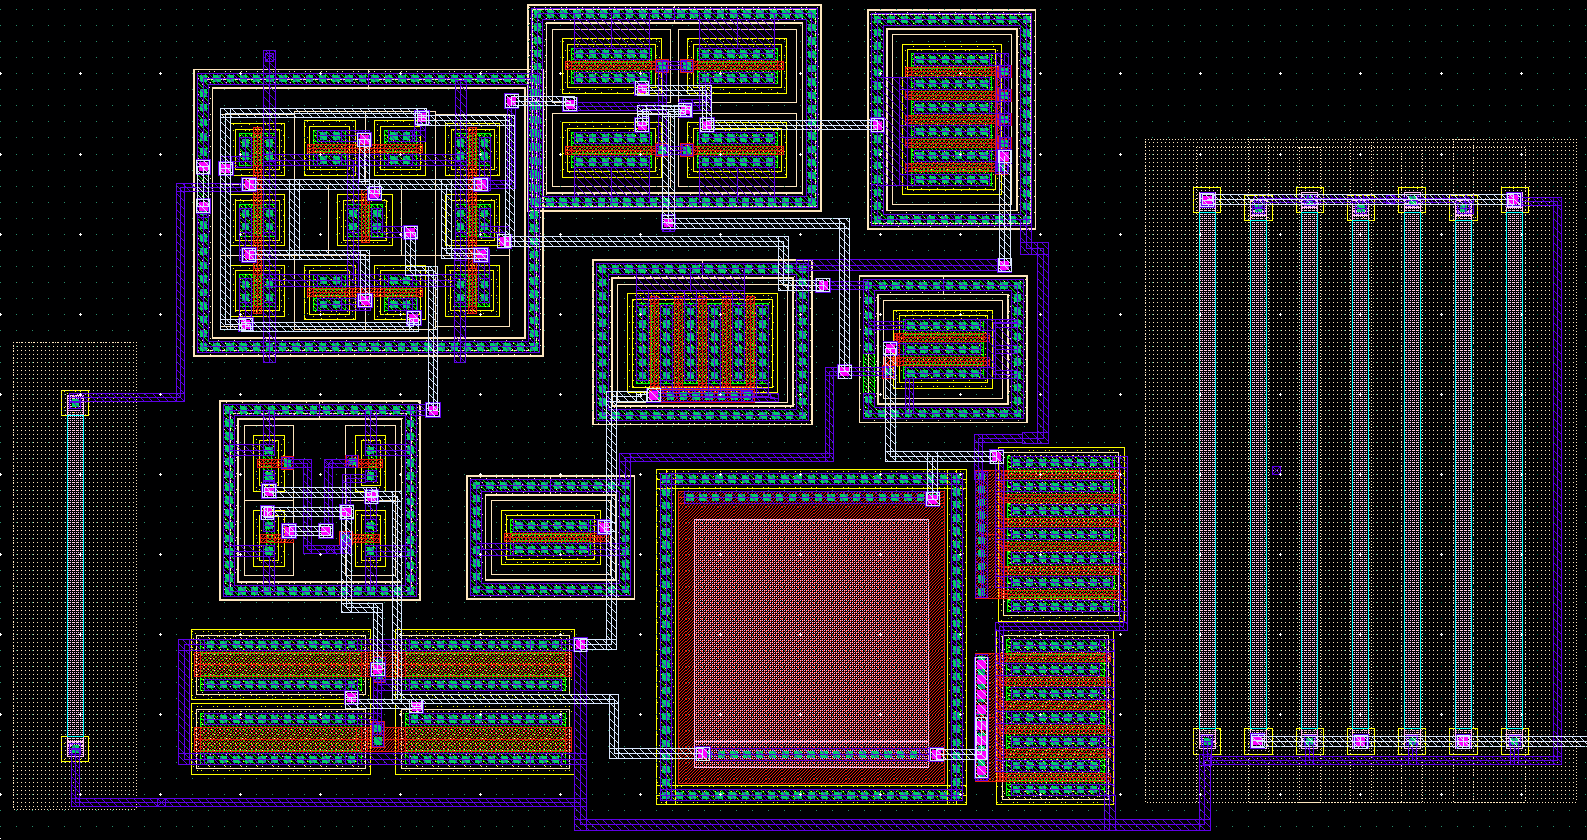
\includegraphics[width=\linewidth-1cm]{layout_g.png}

~

Le ballast:

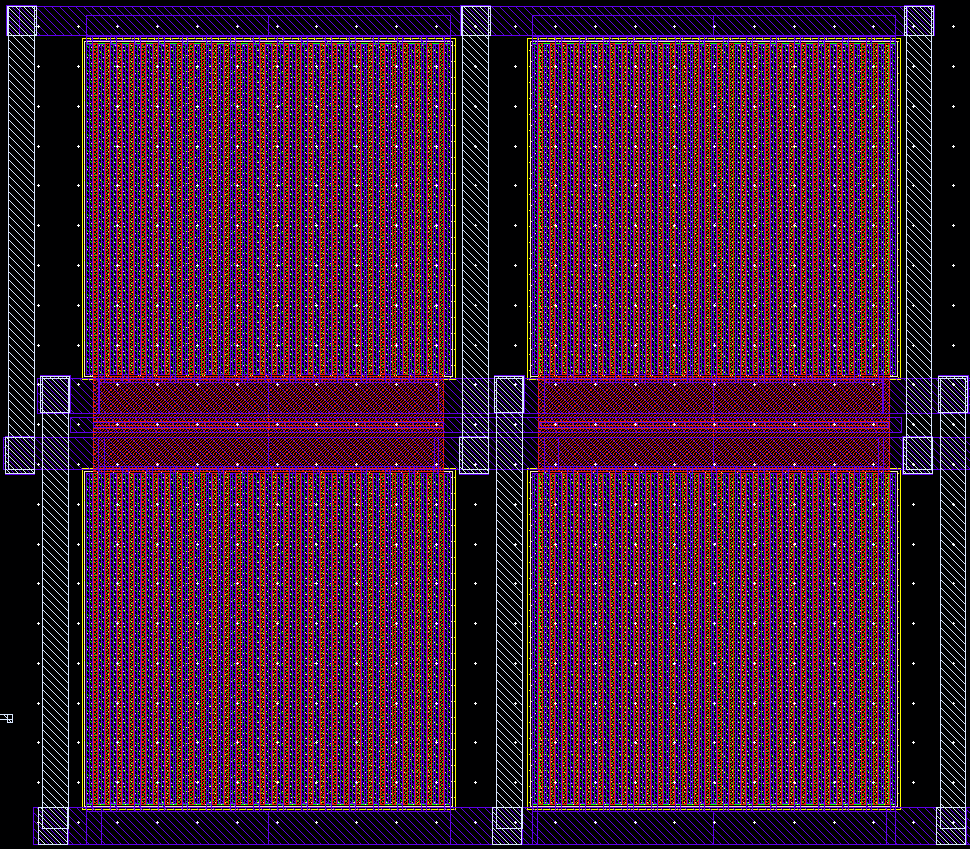
\includegraphics[width=\linewidth-1cm]{layout_d.png}


\subsection{Résultats}

\begin{center}
\begin{tabular}{|l|c|r|}
    \hline
    Paramètre & Unité & \\
    \hline
    Marge de phase & degrès & 73.8 \\
    \hline
    Marge de gain & dB & 21.7 \\
    \hline
    Gain & dB &  79.5 \\
    \hline
    Offset & µV & 4 \\
    \hline
    PSSR & dB & 81.9 \\
    \hline
    Consommation & µA & 498.7 \\
    \hline
    Impédance de sortie & Ω & 6.99 \\
    \hline
\end{tabular}
\end{center}

~

Les résultats ne sont pas si différents, et répondent toujours au cahier des charges.


\section*{Conclusion}

Même si la conception de ce système n’a pas été évidente, la phase de routage a été très intéressante et nous avons beaucoup progressé dans la maîtrise de l’outil Cadence et dans les techniques de routage d’un ASIC.

Le projet dans son ensemble nous a permis d’étudier l’intégralité du processus de conception d’un ASIC Analogique.

L’étape suivante est la réalisation de ce layout en salle blanche, et nous l’avons également vu cette année.

~

Notre circuit répond au cahier des charges, même si n’avons pas eu besoin d’utiliser à outrance un certain nombre des techniques que nous avons vu en cours.

Par exemple, il aurait probablement été très intéressant de cascoder la source de courant de la paire différentielle afin d’augmenter drastiquement son impédance, mais ça n’a pas été nécessaire dans notre cas.

~

Afin d’obtenir un circuit complet, il ne nous resterait plus qu’à fusionner notre layout et celui de l’un des binôme ayant travaillé sur le band-gap avant d’avoir un régulateur linéaire faible puissance et large bande.

On pourrait alors vérifier le fonctionnement global du système, la stabilité et la précision en tension de sa sortie, ainsi que la totalité des points abordés dans le cahier des charges.

\section*{Post Scriptum}

La source \LaTeX de ce rapport est disponible à l’adresse \url{http://bde.saurel.me/rapport_Pierron-Saurel_ASIC.tex}

\end{document}
